\documentclass[../VorlesungMaster.tex]{subfiles}
\begin{document}
%Vorlesung 9 16.11.2017
\section{Nichtlineare Regression}
\subsection{Rückblick: Lineare Regression}
\[ Y= \beta_0 + \beta_1 x_1^{(1)} + ... + \beta_k x_i^{(k)} + \epsilon_i, \; i \in \{1,...,n\} \]
\begin{itemize}
 \item $n$: Anzahl Messungen 
 \item $k$: Anzahl Kovariablen 
 \item $x_i^{(j)}$: Wer der Kovariablen $j$ von Individuum $i$
 \item $\epsilon_i$: zufällige Störungshäufigkeit $\epsilon_i \sim N(0, \sigma^2), \sigma^2 > 0$, unabh.
 \item $\beta_j$: unbekannter, wahrer, zu schätzender Parameter
\end{itemize}
$\rightarrow$ Kleinste Quadrate Methode:
\[ \sum\limits_{i=1}^n \left(y_i - (\beta_0 + \beta_1 x_1^{(1)} + ... + \beta_k x_i^{(k)} \right)^2 \rightarrow min \]

\subsection{Nichtlineare Regression}
\begin{itemize}
 \item häufig nichtlneare Zusammenhänge zwischen abhängiger und unabhängigen Variablen 
	\begin{sloppypar}
	 $\rightarrow$ manchmal aus dem theoretischen Wissen/empirischen Beobachtungen bekannt
	\end{sloppypar}
 \item beschränkter Wertebereich, z.B. $R=[0,1]$ (Wahrscheinlichkeit an einer Krankheit zu erkranken)
 \item diskreter Wertebereich, z.B. $R={0,1}$ (dichotome Zielgröße ``Ja/Nein'')
\end{itemize}

\begin{tikzpicture}
\begin{axis}[%
scatter/classes={%
	a={mark=o,draw=gray}},
xlabel={x},
ylabel={y},
xticklabels={,,},
yticklabels={,,}
]
\addplot[scatter,only marks,%
scatter src=explicit symbolic]%
table[meta=label] {
	x y label
	5 12 a
	6 14 a
	7 16 a
	8 17 a
	9 18 a
	10 18 a
	11 17.5 a
	12 17 a
	13 16 a
	
	15 16 a
	16 18 a
	17 20 a
	18 21 a
	19 22 a
	20 22 a
	21 21 a
	22 20 a
	23 19 a
	
};
\addplot [thick] coordinates { (4,14) (23,21) };
\end{axis}
\end{tikzpicture}
\todo{Man sieht Lineare Regression ist hier schlecht}
\subsubsection{Modell}
\[Y_i = \underbrace{h}_{\text{Funktion i.A. nichtlinear}} \left(\underbrace{x_i^{(1)},...,x_i^{(k)}}_{\text{Kovariablen}};
\underbrace{\theta_1,...,\theta_p}_{\text{(unbekannte Parameter)}} \right) + \epsilon_i, \; i \in \{1,...,n\} \]

$\epsilon_i \sim N(0,\sigma^2) , \sigma^2 >0$, unabhängig

\subsubsection{Beispiele}
Biochemischer Sauerstoffverbrauch von Mikroorganismen
\[h(x;\theta_1,\theta_2) = \theta_1(1-exp(-\theta_2 x)) \]

Cobb-Douglas-Funktion
\[h(x^{(1)},x^{(2)}; \theta_1, \theta_2, \theta_3)= \theta_1(x^{(1)})^{\theta_2} (x^{(2)})^{\theta_3} \]

Polynomiale Regression
\[h(x; \theta_0,..., \theta_p)= \theta_0 + \theta_1 x  + \theta_2 x^2 + ... + \theta_p x^p \]

prinzipiell ``alles möglich'' \\

Wahl/Entscheidung anhand des Wissens über das Problem

\subsection{Linearisierung}
manchmal lässt sich $h$ in einen Ausdruck verwandeln, welcher linear in den transformierten Variablen ist \\
$\rightarrow$ lineare Regression \\
\underline{Beispiel:}
\[ h(x; \theta_1, \theta_2) = \theta_1 x^{\theta_2} \]

\[ \Rightarrow \underbrace{\log h}_{=:  \tilde{h}}(x; \theta_1, \theta_2) = \log \theta_1 + \log x^{\theta_2} \]
\[= \underbrace{\log \theta_1}_{=: \tilde{\theta_1}} + \underbrace{\theta_2}_{=: \tilde{\theta_2}} \underbrace{ \log x }_{=: \tilde{x}} \]
\[ \rightarrow \tilde{h}(\tilde{x};\tilde{\theta_1} \tilde{ \theta_2} ) = \tilde{\theta_1} \tilde{\theta_2} \tilde{x} \]
Lineare Regression
\[ Y_i=\log y_i \]
\[ \rightarrow \tilde{Y_i} = \log y_i = \tilde{h}(\tilde{x_i} \tilde{\theta_1} \tilde{ \theta_2}) + \epsilon_i \]
\[ \tilde{\theta_1} + \tilde{\theta_2} \tilde{x_i} + \epsilon_i, \; i \in \{1,...,n\} \]
$\rightarrow$ Schätzung von $\tilde{\theta_1}$ und $\tilde{\theta_2}$ \\
Aber: $\epsilon_i \sim N(0,\sigma^2), \sigma^2 > 0$, unabh.\\
Rücktransformation:
\[ Y_i = \exp(\tilde{\theta_1} + \tilde{\theta_2} \tilde{x_i} + \epsilon_i ) \]
\[ = \underbrace{\exp(\tilde{\theta_1})}_{=\theta_1} \underbrace{\exp(\tilde{\theta_2}\tilde{x_i})}_{
\substack{= \exp(\theta_2 x_i) \\ = \exp ( \exp ( \tilde{x_i} ))^{\theta_2} \\ = x_i^{\theta_2} }}
\exp(\epsilon_i) \]
\[= \theta_1 x_i^{\theta_2} \exp (\epsilon_i) \]

$\rightarrow$ Durch Transformation betrachtet man ein Modell, in dem sich die Fehler
\begin{itemize}
 \item multiplikativ verhalten
 \item log - normalverteilt sind
\end{itemize}

\[``X \sim LN`` \text{ , falls } `` \log (x) \sim N `` \]

\underline{Vergleich:}
\[ Y_i= \theta_1 x_i^{\theta_2} + \epsilon_i , \; i \in \{1,...,n\} \text{ mit } \epsilon_i \sim N(0, \sigma^2), \sigma^2 > 0 \text{, unabhängig} \]

Linearisierung nur, falls sich die Fehler tatsächlich so wie in der transformierten Variable verhalten \\
$\Rightarrow$ Residuenanalyse

\subsection{Spezielle nichtlineare Situation}

\[Y_i = \underbrace{
\sum_{j=1}^{p} \theta_j h_j (x^{(1)},...,x^{(k)} )}
_{\mathrel{\widehat{=}}  h (x_i^{(1)},...,x_i^{(k)}; \theta_1,..., \theta_p) }
+ \epsilon_i , \; i \in \{1,...,n\} \]

\underline{Beispiele:}
\begin{enumerate} 
 \item $h_j((x_i^{(1)},...,x_i^{(k)}) = x_i^{(j)} \rightarrow$  lineares Modell
 \item $h_j(x_i) = x_i^{j} \rightarrow$ polynomielle Terme
 \item $h_j((x_i^{(1)},...,x_i^{(k)}) = \mathbbm{1}_{[\alpha_j,\alpha_{j+1})} (x_i^{(j)})$ \todo{$\mathbbm{1}$ ist Indikatorfunktion}\\
 $= \begin{cases}
 1, \text{ falls } x_i^{(j)} \in [\alpha_j,\alpha_{j+1}) \\
 0, \text{ falls } x_i^{(j)} \notin [\alpha_j,\alpha_{j+1}) \\
 \end{cases}$
\end{enumerate}

\subsubsection{Polynomiale Regression (Hier:k=1)}
\[Y_i = \theta_0 + \theta_1 x_i^1 +  \theta_2 x_i^2 + ... +  \theta_p x_i^p + \epsilon_i, \; i \in \{1,...,n\} \]
\todo{Oszi bild}

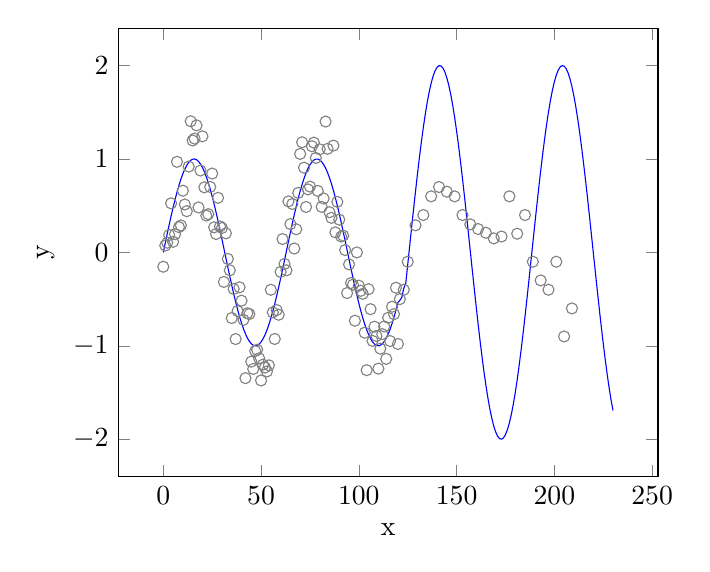
\begin{tikzpicture}
\begin{axis}[%
scatter/classes={%
	a={mark=o,draw=gray}},
xlabel={x},
ylabel={y}
%,
%xticklabels={,,},
%yticklabels={,,}
]
\addplot[scatter,only marks,%
scatter src=explicit symbolic]%
table[meta=label] {
	x y label
0 -0.153598481556401  a
1 0.073583842847978  a
2 0.10389364452171  a
3 0.186267113992389  a
4 0.52527384219649  a
5 0.112936649511624  a
6 0.195148680164532  a
7 0.969726716445442  a
8 0.270429246127571  a
9 0.288292071765007  a
10 0.660444693472895  a
11 0.512673438624097  a
12 0.441350472118466  a
13 0.918543608896422  a
14 1.40390367343846  a
15 1.19766597575237  a
16 1.21809212723937  a
17 1.35964192321696  a
18 0.480920001610398  a
19 0.876400165916276  a
20 1.24273100042559  a
21 0.69634472843208  a
22 0.393930384502455  a
23 0.409371241171787  a
24 0.700672680772686  a
25 0.843915121744734  a
26 0.26855643443212  a
27 0.196910684828808  a
28 0.58397179550192  a
29 0.277612332851624  a
30 0.261196727265694  a
31 -0.316064773989609  a
32 0.204179484175176  a
33 -0.0700189241743814  a
34 -0.191866644189935  a
35 -0.702653568916078  a
36 -0.391797129708066  a
37 -0.927683507660596  a
38 -0.627872377028343  a
39 -0.373623253775458  a
40 -0.51682582308509  a
41 -0.721734043231002  a
42 -1.34605777578016  a
43 -0.651293807907056  a
44 -0.659866508832492  a
45 -1.16937402152145  a
46 -1.24765467246416  a
47 -1.0561926394579  a
48 -1.0424331881531  a
49 -1.1337060341824  a
50 -1.37099184864636  a
51 -1.20129418879613  a
52 -1.23220823840634  a
53 -1.27441440449963  a
54 -1.20911279380395  a
55 -0.400334340597975  a
56 -0.641800695498822  a
57 -0.926682875919358  a
58 -0.617602414738482  a
59 -0.667398500997437  a
60 -0.208974790237829  a
61 0.142755064785921  a
62 -0.123397054789895  a
63 -0.191620694310757  a
64 0.546173777479603  a
65 0.302779761504633  a
66 0.518496018518044  a
67 0.0413399797017886  a
68 0.247443479406016  a
69 0.636836718244773  a
70 1.05444791969086  a
71 1.17872428571273  a
72 0.907081899493535  a
73 0.485967477997869  a
74 0.674098773897014  a
75 0.704245298843892  a
76 1.13647987799027  a
77 1.17501625103126  a
78 1.01096408279202  a
79 0.65828653583866  a
80 1.10327543697211  a
81 0.487291656272316  a
82 0.577043921287986  a
83 1.40049109034138  a
84 1.10866514347412  a
85 0.4300360910118  a
86 0.369918816640654  a
87 1.14303561077855  a
88 0.214336417228505  a
89 0.540859709750052  a
90 0.35053879609108  a
91 0.169554660445458  a
92 0.17950010874048  a
93 0.0249355767866046  a
94 -0.435242791178949  a
95 -0.128343795808318  a
96 -0.327568836782512  a
97 -0.34557547135639  a
98 -0.731545219152139  a
99 -0.000331437799878209  a
100 -0.356502871402407  a
101 -0.411120454008792  a
102 -0.443075264224896  a
103 -0.859489313219177  a
104 -1.26079604343652  a
105 -0.394209446969486  a
106 -0.607680788584896  a
107 -0.947322925806252  a
108 -0.795221191737129  a
109 -0.894400926587093  a
110 -1.2443188038784  a
111 -1.03026062913432  a
112 -0.874761627911695  a
113 -0.792999976334144  a
114 -1.13991377526188  a
115 -0.700012684450224  a
116 -0.948881983897702  a
117 -0.581700829095467  a
118 -0.660890968766382  a
119 -0.378357931855586  a
120 -0.980085463898992  a

121 -0.5  a
123 -0.4  a
125 -0.1  a
129 0.29  a
133 0.4  a
137 0.6 a
141 0.7 a
145 0.65  a
149 0.6  a
153 0.4  a
157 0.3  a
161 0.25  a
165 0.21  a
169 0.15  a
173 0.17  a
177 0.6 a
181 0.2  a
185 0.4  a
189 -0.1  a
193 -0.3  a
197 -0.4  a
201 -0.1  a
205 -0.9  a
209 -0.6  a

};
\addplot [blue] coordinates{
( 0 , 0 )
( 1 , 0.0998334166468282 )
( 2 , 0.198669330795061 )
( 3 , 0.29552020666134 )
( 4 , 0.389418342308651 )
( 5 , 0.479425538604203 )
( 6 , 0.564642473395035 )
( 7 , 0.644217687237691 )
( 8 , 0.717356090899523 )
( 9 , 0.783326909627483 )
( 10 , 0.841470984807897 )
( 11 , 0.891207360061435 )
( 12 , 0.932039085967226 )
( 13 , 0.963558185417193 )
( 14 , 0.98544972998846 )
( 15 , 0.997494986604054 )
( 16 , 0.999573603041505 )
( 17 , 0.991664810452469 )
( 18 , 0.973847630878195 )
( 19 , 0.946300087687414 )
( 20 , 0.909297426825682 )
( 21 , 0.863209366648874 )
( 22 , 0.80849640381959 )
( 23 , 0.74570521217672 )
( 24 , 0.675463180551151 )
( 25 , 0.598472144103957 )
( 26 , 0.515501371821464 )
( 27 , 0.42737988023383 )
( 28 , 0.334988150155905 )
( 29 , 0.239249329213982 )
( 30 , 0.141120008059867 )
( 31 , 0.0415806624332905 )
( 32 , -0.0583741434275801 )
( 33 , -0.157745694143249 )
( 34 , -0.255541102026832 )
( 35 , -0.35078322768962 )
( 36 , -0.442520443294852 )
( 37 , -0.529836140908493 )
( 38 , -0.611857890942719 )
( 39 , -0.687766159183974 )
( 40 , -0.756802495307928 )
( 41 , -0.818277111064411 )
( 42 , -0.871575772413588 )
( 43 , -0.916165936749455 )
( 44 , -0.951602073889516 )
( 45 , -0.977530117665097 )
( 46 , -0.993691003633465 )
( 47 , -0.999923257564101 )
( 48 , -0.996164608835841 )
( 49 , -0.982452612624332 )
( 50 , -0.958924274663138 )
( 51 , -0.925814682327732 )
( 52 , -0.883454655720153 )
( 53 , -0.832267442223901 )
( 54 , -0.772764487555987 )
( 55 , -0.705540325570392 )
( 56 , -0.631266637872321 )
( 57 , -0.550685542597638 )
( 58 , -0.464602179413757 )
( 59 , -0.373876664830236 )
( 60 , -0.279415498198926 )
( 61 , -0.182162504272095 )
( 62 , -0.0830894028174964 )
( 63 , 0.0168139004843506 )
( 64 , 0.116549204850494 )
( 65 , 0.215119988087816 )
( 66 , 0.311541363513379 )
( 67 , 0.404849920616598 )
( 68 , 0.494113351138609 )
( 69 , 0.5784397643882 )
( 70 , 0.656986598718789 )
( 71 , 0.728969040125876 )
( 72 , 0.793667863849153 )
( 73 , 0.850436620628565 )
( 74 , 0.898708095811627 )
( 75 , 0.937999976774739 )
( 76 , 0.967919672031487 )
( 77 , 0.988168233877 )
( 78 , 0.998543345374605 )
( 79 , 0.998941341839772 )
( 80 , 0.989358246623382 )
( 81 , 0.969889810845086 )
( 82 , 0.940730556679773 )
( 83 , 0.902171833756293 )
( 84 , 0.85459890808828 )
( 85 , 0.79848711262349 )
( 86 , 0.734397097874113 )
( 87 , 0.662969230082182 )
( 88 , 0.584917192891762 )
( 89 , 0.501020856457885 )
( 90 , 0.412118485241757 )
( 91 , 0.319098362349352 )
( 92 , 0.222889914100246 )
( 93 , 0.124454423507062 )
( 94 , 0.0247754254533578 )
( 95 , -0.0751511204618093 )
( 96 , -0.174326781222981 )
( 97 , -0.271760626410944 )
( 98 , -0.366479129251928 )
( 99 , -0.457535893775321 )
( 100 , -0.54402111088937 )
( 101 , -0.625070648892883 )
( 102 , -0.699874687593544 )
( 103 , -0.767685809763582 )
( 104 , -0.827826469085654 )
( 105 , -0.87969575997167 )
( 106 , -0.922775421612807 )
( 107 , -0.956635016270188 )
( 108 , -0.980936230066492 )
( 109 , -0.995436253306377 )
( 110 , -0.999990206550703 )
( 111 , -0.994552588203989 )
( 112 , -0.979177729151317 )
( 113 , -0.954019249902089 )
( 114 , -0.919328525664676 )
( 115 , -0.875452174688429 )
( 116 , -0.822828594968708 )
( 117 , -0.761983583919032 )
( 118 , -0.693525084777122 )
( 119 , -0.618137112237033 )
( 120 , -0.536572918000435 )
( 121 , -0.5129069203 )
( 122 , -0.48 )
( 123 , -0.3826463582731602 )
( 124 , -0.331208350896619 )
( 125 , -0.132643794702401 )
( 126 , 0.0672460944422734 )
( 127 , 0.266464082839884 )
( 128 , 0.463019650203078 )
( 129 , 0.654948878275386 )
( 130 , 0.840334073653282 )
( 131 , 1.01732292874475 )
( 132 , 1.18414702941445 )
( 133 , 1.3391395243932 )
( 134 , 1.4807517799049 )
( 135 , 1.60756885310324 )
( 136 , 1.71832362971299 )
( 137 , 1.81190948461692 )
( 138 , 1.88739133888821 )
( 139 , 1.94401500278995 )
( 140 , 1.98121471138974 )
( 141 , 1.99861877749584 )
( 142 , 1.99605330543272 )
( 143 , 1.97354392854923 )
( 144 , 1.93131555309855 )
( 145 , 1.86979011104937 )
( 146 , 1.78958234428101 )
( 147 , 1.69149366228587 )
( 148 , 1.57650413475063 )
( 149 , 1.44576269902395 )
( 150 , 1.30057568031423 )
( 151 , 1.14239373931998 )
( 152 , 0.972797377707599 )
( 153 , 0.793481146261224 )
( 154 , 0.606236713491405 )
( 155 , 0.412934963875593 )
( 156 , 0.215507304598888 )
( 157 , 0.0159263675718747 )
( 158 , -0.183813700455363 )
( 159 , -0.381717162748379 )
( 160 , -0.575806633330131 )
( 161 , -0.764142834368018 )
( 162 , -0.944843972796932 )
( 163 , -1.11610454257356 )
( 164 , -1.27621336469589 )
( 165 , -1.42357068473825 )
( 166 , -1.5567041570686 )
( 167 , -1.67428355603949 )
( 168 , -1.77513406716301 )
( 169 , -1.85824802546874 )
( 170 , -1.92279498375911 )
( 171 , -1.96813001016329 )
( 172 , -1.99380013208319 )
( 173 , -1.99954886214602 )
( 174 , -1.98531876094127 )
( 175 , -1.95125201093632 )
( 176 , -1.89768899583625 )
( 177 , -1.82516489958237 )
( 178 , -1.73440435897116 )
( 179 , -1.62631422332298 )
( 180 , -1.50197449354335 )
( 181 , -1.362627531111 )
( 182 , -1.20966564481257 )
( 183 , -1.04461717925346 )
( 184 , -0.869131244143794 )
( 185 , -0.684961236939225 )
( 186 , -0.493947323473242 )
( 187 , -0.297998051628398 )
( 188 , -0.0990712817567348 )
( 189 , 0.100845375613622 )
( 190 , 0.299754419325905 )
( 191 , 0.49566841596592 )
( 192 , 0.686629857639791 )
( 193 , 0.870730720745786 )
( 194 , 1.04613153031539 )
( 195 , 1.2110797394392 )
( 196 , 1.36392724013627 )
( 197 , 1.5031468307043 )
( 198 , 1.62734747501421 )
( 199 , 1.73528820128333 )
( 200 , 1.82589050145526 )
( 201 , 1.89824910729579 )
( 202 , 1.95164103553395 )
( 203 , 1.98553281167181 )
( 204 , 1.99958580028534 )
( 205 , 1.9936595885576 )
( 206 , 1.96781338923723 )
( 207 , 1.92230544900423 )
( 208 , 1.85759046815448 )
( 209 , 1.7743150573847 )
( 210 , 1.67331127707211 )
( 211 , 1.55558832360219 )
( 212 , 1.42232244581196 )
( 213 , 1.27484519230048 )
( 214 , 1.11463010703532 )
( 215 , 0.943278006188392 )
( 216 , 0.76250098330988 )
( 217 , 0.57410530265545 )
( 218 , 0.379973351590875 )
( 219 , 0.182044832399696 )
( 220 , -0.0177026185808078 )
( 221 , -0.21727319084816 )
( 222 , -0.414672841213524 )
( 223 , -0.607929217622094 )
( 224 , -0.795111366242866 )
( 225 , -0.974349024921019 )
( 226 , -1.14385131021913 )
( 227 , -1.3019246113325 )
( 228 , -1.44698951208849 )
( 229 , -1.57759657195083 )
( 230 , -1.69244080835034 )
};
\end{axis}
\end{tikzpicture}
p groß:
\begin{itemize}
 \item bessere Anpassung an Daten
 \item schlechtes Verhalten am Rand(Oszillation)
\end{itemize}

\subsubsection{Stückweise Regression (Hier:k=1)}
\[Y_i= \sum\limits_{j=1}^{p} \mathbbm{1}_{[\alpha_j,\alpha_{j+1})} (x_i) + \epsilon_i  \; i \in \{1,...,n\} \]
stückweise Approximation mit konstanten Funktionen
\todo{Stufen Bild}

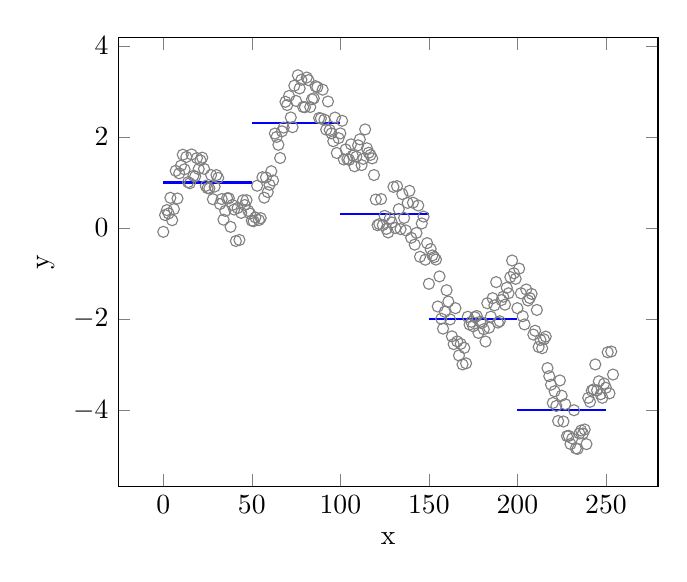
\begin{tikzpicture}
\begin{axis}[%
scatter/classes={%
	a={mark=o,draw=gray}},
xlabel={x},
ylabel={y}
%,
%xticklabels={,,},
%yticklabels={,,}
]
\addplot[scatter,only marks,%
scatter src=explicit symbolic]%
table[meta=label] {
	x y label
0 -0.0835160242859274  a
1 0.285568934387078  a
2 0.394579101186943  a
3 0.319456011084284  a
4 0.663787821139718  a
5 0.172388397197294  a
6 0.415525883567572  a
7 1.2558843677376  a
8 0.648844252387028  a
9 1.20117942302646  a
10 1.37047603500141  a
11 1.60972337793055  a
12 1.28911192846088  a
13 1.56031080227344  a
14 1.00638248369854  a
15 0.984246086186816  a
16 1.61625921176936  a
17 1.14765390737154  a
18 1.13367303859185  a
19 1.53545813877587  a
20 1.29462647613912  a
21 1.48594938329369  a
22 1.54546652597812  a
23 1.30075626330351  a
24 0.924780725901792  a
25 0.876653467885566  a
26 0.868665008436964  a
27 1.16370842893904  a
28 0.632732011300313  a
29 0.910259724400004  a
30 1.16219661138681  a
31 1.1008670138421  a
32 0.526987032463432  a
33 0.636180665523263  a
34 0.183851565842274  a
35 0.375588325804044  a
36 0.653835219246611  a
37 0.653046301882522  a
38 0.025952382432643  a
39 0.506237835066696  a
40 0.406508096522012  a
41 -0.284979202944553  a
42 0.441617462853366  a
43 -0.261760379385229  a
44 0.333222419824161  a
45 0.608838475955039  a
46 0.506281967150246  a
47 0.612056507974025  a
48 0.377464089267289  a
49 0.318273150014862  a
50 0.160728241545451  a
51 0.149920991073773  a
52 0.234019446415594  a
53 0.929124473902112  a
54 0.174356963261225  a
55 0.21750907289469  a
56 1.11559149778506  a
57 0.666788690482064  a
58 1.1108994162566  a
59 0.789282054504515  a
60 0.949495578473449  a
61 1.24609024287059  a
62 1.0439689383038  a
63 2.0738032175923  a
64 2.00021885098137  a
65 1.82646297140817  a
66 1.53750375053874  a
67 2.12319951961666  a
68 2.20452596942365  a
69 2.77103151086561  a
70 2.6996241669188  a
71 2.89934425580715  a
72 2.42736370696646  a
73 2.21425717093992  a
74 3.1240761414546  a
75 2.79047215541272  a
76 3.35357788576053  a
77 3.06462581275212  a
78 3.25621667858734  a
79 2.65606834912304  a
80 2.65170938178788  a
81 3.30359897359816  a
82 3.24693918137054  a
83 2.6567775906426  a
84 2.82500878652476  a
85 2.84711065352786  a
86 3.11358688446847  a
87 3.09279924916506  a
88 2.41591744253837  a
89 2.40630980085128  a
90 3.037289616929  a
91 2.37940869990215  a
92 2.15993843587786  a
93 2.77768389042592  a
94 2.15155270292113  a
95 2.07769601288223  a
96 1.90690445719062  a
97 2.42502603913297  a
98 1.64768546107142  a
99 1.97305051518811  a
100 2.07749159503648  a
101 2.35429938200758  a
102 1.50443150226202  a
103 1.72591064257131  a
104 1.51359098360733  a
105 1.49705886968687  a
106 1.83741092845341  a
107 1.5901074953636  a
108 1.35674404320374  a
109 1.56577833681282  a
110 1.81587205071571  a
111 1.94639450565719  a
112 1.38145985457197  a
113 1.518824266064  a
114 2.16497044046184  a
115 1.75152454886146  a
116 1.65343895  a
117 1.60452768713676  a
118 1.52887  a
119 1.16346422492016  a
120 0.62567950418891  a
121 0.0617660779505969  a
122 0.0874130559773345  a
123 0.636246310715329  a
124 0.065931420837905  a
125 0.266933389091442  a
126 -0.0187439220090775  a
127 -0.0965087727913103  a
128 0.215647966794353  a
129 0.123426863029565  a
130 0.903224120057837  a
131 0.000716092782753586  a
132 0.919853450296996  a
133 0.414521310074015  a
134 -0.0239557141624512  a
135 0.744421694481854  a
136 0.222568307115783  a
137 -0.0516699323132284  a
138 0.552116727206714  a
139 0.816264725585684  a
140 -0.21322574585225  a
141 0.556972587703088  a
142 -0.364064165652314  a
143 -0.106444775224954  a
144 0.494334064171592  a
145 -0.630523341009548  a
146 0.10091122698353  a
147 0.251485628293903  a
148 -0.694754468553538  a
149 -0.330634462175158  a
150 -1.22386964907777  a
151 -0.460814841690383  a
152 -0.600979046426481  a
153 -0.637546556795358  a
154 -0.691924402320308  a
155 -1.72239511476575  a
156 -1.06126261095336  a
157 -1.99039620129457  a
158 -2.20762669760753  a
159 -1.83641583911109  a
160 -1.36503154749765  a
161 -1.61305348642141  a
162 -2.00492559158406  a
163 -2.37670630930511  a
164 -2.54764689092713  a
165 -1.75859506579145  a
166 -2.48808753905506  a
167 -2.79628780843111  a
168 -2.54246577581102  a
169 -2.99359631841596  a
170 -2.63023243383767  a
171 -2.96961812391381  a
172 -1.94707443090953  a
173 -2.1191392756945  a
174 -2.05823633738729  a
175 -2.15585085439569  a
176 -1.95754764171644  a
177 -1.92977651096822  a
178 -2.30121753374042  a
179 -2.05512077363031  a
180 -2.07841025295281  a
181 -2.22054002107119  a
182 -2.49052823895731  a
183 -1.6500262714702  a
184 -2.18659764135757  a
185 -1.9456184006092  a
186 -1.53888803367664  a
187 -1.69660847681546  a
188 -1.18698964913457  a
189 -2.07456341874383  a
190 -2.0453887798746  a
191 -1.58061223276717  a
192 -1.5072742650618  a
193 -1.68141803383867  a
194 -1.31140627053556  a
195 -1.43173297908125  a
196 -1.07619946377905  a
197 -0.712681362673109  a
198 -0.992644450979355  a
199 -1.11508761295528  a
200 -1.75934427392106  a
201 -0.889907055516884  a
202 -1.43146357298287  a
203 -1.93476802335877  a
204 -2.11464198354733  a
205 -1.34866493998177  a
206 -1.59040358835008  a
207 -1.5359533704895  a
208 -1.4454749544856  a
209 -2.33825520330615  a
210 -2.25373298405192  a
211 -1.79731093417145  a
212 -2.61019870508052  a
213 -2.4560855332043  a
214 -2.63723998084539  a
215 -2.44225632768435  a
216 -2.38277372974931  a
217 -3.07383448990287  a
218 -3.25058158518176  a
219 -3.43847567938352  a
220 -3.8396760472169  a
221 -3.58253451343706  a
222 -3.90411063143155  a
223 -4.23479710460466  a
224 -3.34476936812928  a
225 -3.67984879142745  a
226 -4.2454842520664  a
227 -3.86529398324425  a
228 -4.56723044702059  a
229 -4.5617398320318  a
230 -4.74043676227416  a
231 -4.61830041731139  a
232 -3.998853175195  a
233 -4.83718294916592  a
234 -4.84698107957931  a
235 -4.50950485401081  a
236 -4.44364534968019  a
237 -4.5106354052397  a
238 -4.42164548253201  a
239 -4.74294782679374  a
240 -3.72734344634738  a
241 -3.81452325776479  a
242 -3.5682339220494  a
243 -3.54258694402267  a
244 -2.99375368928467  a
245 -3.56406857916209  a
246 -3.36306661090856  a
247 -3.64874392200908  a
248 -3.72650877279131  a
249 -3.41435203320565  a
250 -3.50657313697043  a
251 -2.72677587994216  a
252 -3.62928390721725  a
253 -2.710146549703  a
254 -3.21547868992598  a


};
\addplot[blue, thick] coordinates {(0,1) (50,1)};
\addplot[blue, thick] coordinates {(50,2.3) (100,2.3)};
\addplot[blue, thick] coordinates {(100,0.3) (150,0.3)};
\addplot[blue, thick] coordinates {(150,-2) (200,-2)};
\addplot[blue, thick] coordinates {(200,-4) (250,-4)};
\end{axis}
\end{tikzpicture}

Erweiterung: lineare /quadratische/kubische/.. Funktionen

\underline{Beispiel:}
\[Y_i= \sum\limits_{j=1}^{p}(a_j x_i^3 + b_j x_i^2 + c_j x_i + d_j) \mathbbm{1}_{[\alpha_j,\alpha_{j+1})} (x_i) + \epsilon_i  \; i \in \{1,...,n\} \]
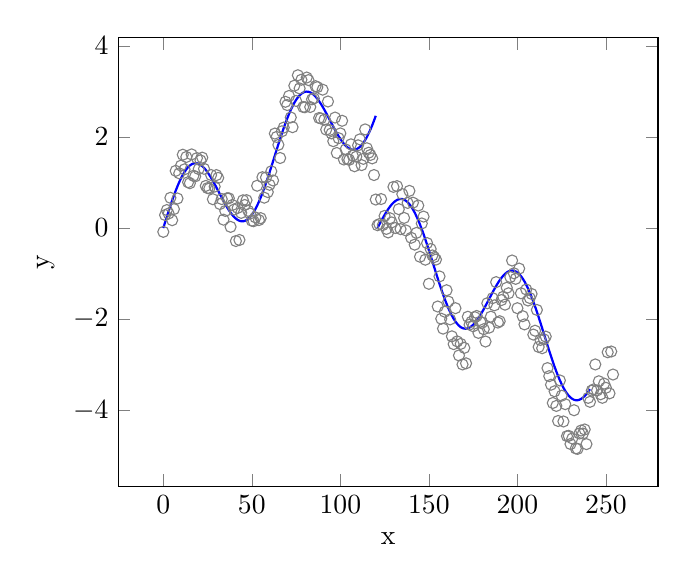
\begin{tikzpicture}
\begin{axis}[%
scatter/classes={%
	a={mark=o,draw=gray}},
xlabel={x},
ylabel={y}
%,
%xticklabels={,,},
%yticklabels={,,}
]
\addplot[scatter,only marks,%
scatter src=explicit symbolic]%
table[meta=label] {
	x y label
0 -0.0835160242859274  a
1 0.285568934387078  a
2 0.394579101186943  a
3 0.319456011084284  a
4 0.663787821139718  a
5 0.172388397197294  a
6 0.415525883567572  a
7 1.2558843677376  a
8 0.648844252387028  a
9 1.20117942302646  a
10 1.37047603500141  a
11 1.60972337793055  a
12 1.28911192846088  a
13 1.56031080227344  a
14 1.00638248369854  a
15 0.984246086186816  a
16 1.61625921176936  a
17 1.14765390737154  a
18 1.13367303859185  a
19 1.53545813877587  a
20 1.29462647613912  a
21 1.48594938329369  a
22 1.54546652597812  a
23 1.30075626330351  a
24 0.924780725901792  a
25 0.876653467885566  a
26 0.868665008436964  a
27 1.16370842893904  a
28 0.632732011300313  a
29 0.910259724400004  a
30 1.16219661138681  a
31 1.1008670138421  a
32 0.526987032463432  a
33 0.636180665523263  a
34 0.183851565842274  a
35 0.375588325804044  a
36 0.653835219246611  a
37 0.653046301882522  a
38 0.025952382432643  a
39 0.506237835066696  a
40 0.406508096522012  a
41 -0.284979202944553  a
42 0.441617462853366  a
43 -0.261760379385229  a
44 0.333222419824161  a
45 0.608838475955039  a
46 0.506281967150246  a
47 0.612056507974025  a
48 0.377464089267289  a
49 0.318273150014862  a
50 0.160728241545451  a
51 0.149920991073773  a
52 0.234019446415594  a
53 0.929124473902112  a
54 0.174356963261225  a
55 0.21750907289469  a
56 1.11559149778506  a
57 0.666788690482064  a
58 1.1108994162566  a
59 0.789282054504515  a
60 0.949495578473449  a
61 1.24609024287059  a
62 1.0439689383038  a
63 2.0738032175923  a
64 2.00021885098137  a
65 1.82646297140817  a
66 1.53750375053874  a
67 2.12319951961666  a
68 2.20452596942365  a
69 2.77103151086561  a
70 2.6996241669188  a
71 2.89934425580715  a
72 2.42736370696646  a
73 2.21425717093992  a
74 3.1240761414546  a
75 2.79047215541272  a
76 3.35357788576053  a
77 3.06462581275212  a
78 3.25621667858734  a
79 2.65606834912304  a
80 2.65170938178788  a
81 3.30359897359816  a
82 3.24693918137054  a
83 2.6567775906426  a
84 2.82500878652476  a
85 2.84711065352786  a
86 3.11358688446847  a
87 3.09279924916506  a
88 2.41591744253837  a
89 2.40630980085128  a
90 3.037289616929  a
91 2.37940869990215  a
92 2.15993843587786  a
93 2.77768389042592  a
94 2.15155270292113  a
95 2.07769601288223  a
96 1.90690445719062  a
97 2.42502603913297  a
98 1.64768546107142  a
99 1.97305051518811  a
100 2.07749159503648  a
101 2.35429938200758  a
102 1.50443150226202  a
103 1.72591064257131  a
104 1.51359098360733  a
105 1.49705886968687  a
106 1.83741092845341  a
107 1.5901074953636  a
108 1.35674404320374  a
109 1.56577833681282  a
110 1.81587205071571  a
111 1.94639450565719  a
112 1.38145985457197  a
113 1.518824266064  a
114 2.16497044046184  a
115 1.75152454886146  a
116 1.65343895  a
117 1.60452768713676  a
118 1.52887  a
119 1.16346422492016  a
120 0.62567950418891  a
121 0.0617660779505969  a
122 0.0874130559773345  a
123 0.636246310715329  a
124 0.065931420837905  a
125 0.266933389091442  a
126 -0.0187439220090775  a
127 -0.0965087727913103  a
128 0.215647966794353  a
129 0.123426863029565  a
130 0.903224120057837  a
131 0.000716092782753586  a
132 0.919853450296996  a
133 0.414521310074015  a
134 -0.0239557141624512  a
135 0.744421694481854  a
136 0.222568307115783  a
137 -0.0516699323132284  a
138 0.552116727206714  a
139 0.816264725585684  a
140 -0.21322574585225  a
141 0.556972587703088  a
142 -0.364064165652314  a
143 -0.106444775224954  a
144 0.494334064171592  a
145 -0.630523341009548  a
146 0.10091122698353  a
147 0.251485628293903  a
148 -0.694754468553538  a
149 -0.330634462175158  a
150 -1.22386964907777  a
151 -0.460814841690383  a
152 -0.600979046426481  a
153 -0.637546556795358  a
154 -0.691924402320308  a
155 -1.72239511476575  a
156 -1.06126261095336  a
157 -1.99039620129457  a
158 -2.20762669760753  a
159 -1.83641583911109  a
160 -1.36503154749765  a
161 -1.61305348642141  a
162 -2.00492559158406  a
163 -2.37670630930511  a
164 -2.54764689092713  a
165 -1.75859506579145  a
166 -2.48808753905506  a
167 -2.79628780843111  a
168 -2.54246577581102  a
169 -2.99359631841596  a
170 -2.63023243383767  a
171 -2.96961812391381  a
172 -1.94707443090953  a
173 -2.1191392756945  a
174 -2.05823633738729  a
175 -2.15585085439569  a
176 -1.95754764171644  a
177 -1.92977651096822  a
178 -2.30121753374042  a
179 -2.05512077363031  a
180 -2.07841025295281  a
181 -2.22054002107119  a
182 -2.49052823895731  a
183 -1.6500262714702  a
184 -2.18659764135757  a
185 -1.9456184006092  a
186 -1.53888803367664  a
187 -1.69660847681546  a
188 -1.18698964913457  a
189 -2.07456341874383  a
190 -2.0453887798746  a
191 -1.58061223276717  a
192 -1.5072742650618  a
193 -1.68141803383867  a
194 -1.31140627053556  a
195 -1.43173297908125  a
196 -1.07619946377905  a
197 -0.712681362673109  a
198 -0.992644450979355  a
199 -1.11508761295528  a
200 -1.75934427392106  a
201 -0.889907055516884  a
202 -1.43146357298287  a
203 -1.93476802335877  a
204 -2.11464198354733  a
205 -1.34866493998177  a
206 -1.59040358835008  a
207 -1.5359533704895  a
208 -1.4454749544856  a
209 -2.33825520330615  a
210 -2.25373298405192  a
211 -1.79731093417145  a
212 -2.61019870508052  a
213 -2.4560855332043  a
214 -2.63723998084539  a
215 -2.44225632768435  a
216 -2.38277372974931  a
217 -3.07383448990287  a
218 -3.25058158518176  a
219 -3.43847567938352  a
220 -3.8396760472169  a
221 -3.58253451343706  a
222 -3.90411063143155  a
223 -4.23479710460466  a
224 -3.34476936812928  a
225 -3.67984879142745  a
226 -4.2454842520664  a
227 -3.86529398324425  a
228 -4.56723044702059  a
229 -4.5617398320318  a
230 -4.74043676227416  a
231 -4.61830041731139  a
232 -3.998853175195  a
233 -4.83718294916592  a
234 -4.84698107957931  a
235 -4.50950485401081  a
236 -4.44364534968019  a
237 -4.5106354052397  a
238 -4.42164548253201  a
239 -4.74294782679374  a
240 -3.72734344634738  a
241 -3.81452325776479  a
242 -3.5682339220494  a
243 -3.54258694402267  a
244 -2.99375368928467  a
245 -3.56406857916209  a
246 -3.36306661090856  a
247 -3.64874392200908  a
248 -3.72650877279131  a
249 -3.41435203320565  a
250 -3.50657313697043  a
251 -2.72677587994216  a
252 -3.62928390721725  a
253 -2.710146549703  a
254 -3.21547868992598  a


};
\addplot[blue, thick] coordinates {
( 0 , 0 )
( 1 , 0.124833416646828 )
( 2 , 0.248669330795061 )
( 3 , 0.37052020666134 )
( 4 , 0.489418342308651 )
( 5 , 0.604425538604203 )
( 6 , 0.714642473395036 )
( 7 , 0.819217687237691 )
( 8 , 0.917356090899523 )
( 9 , 1.00832690962748 )
( 10 , 1.0914709848079 )
( 11 , 1.16620736006144 )
( 12 , 1.23203908596723 )
( 13 , 1.28855818541719 )
( 14 , 1.33544972998846 )
( 15 , 1.37249498660405 )
( 16 , 1.39957360304151 )
( 17 , 1.41666481045247 )
( 18 , 1.4238476308782 )
( 19 , 1.42130008768741 )
( 20 , 1.40929742682568 )
( 21 , 1.38820936664887 )
( 22 , 1.35849640381959 )
( 23 , 1.32070521217672 )
( 24 , 1.27546318055115 )
( 25 , 1.22347214410396 )
( 26 , 1.16550137182146 )
( 27 , 1.10237988023383 )
( 28 , 1.0349881501559 )
( 29 , 0.964249329213982 )
( 30 , 0.891120008059867 )
( 31 , 0.816580662433291 )
( 32 , 0.74162585657242 )
( 33 , 0.667254305856751 )
( 34 , 0.594458897973168 )
( 35 , 0.52421677231038 )
( 36 , 0.457479556705148 )
( 37 , 0.395163859091507 )
( 38 , 0.338142109057281 )
( 39 , 0.287233840816026 )
( 40 , 0.243197504692072 )
( 41 , 0.206722888935589 )
( 42 , 0.178424227586412 )
( 43 , 0.158834063250545 )
( 44 , 0.148397926110484 )
( 45 , 0.147469882334903 )
( 46 , 0.156308996366536 )
( 47 , 0.175076742435899 )
( 48 , 0.20383539116416 )
( 49 , 0.242547387375668 )
( 50 , 0.291075725336862 )
( 51 , 0.349185317672268 )
( 52 , 0.416545344279847 )
( 53 , 0.492732557776099 )
( 54 , 0.577235512444013 )
( 55 , 0.669459674429608 )
( 56 , 0.768733362127679 )
( 57 , 0.874314457402362 )
( 58 , 0.985397820586244 )
( 59 , 1.10112333516976 )
( 60 , 1.22058450180107 )
( 61 , 1.34283749572791 )
( 62 , 1.4669105971825 )
( 63 , 1.59181390048435 )
( 64 , 1.71654920485049 )
( 65 , 1.84011998808782 )
( 66 , 1.96154136351338 )
( 67 , 2.0798499206166 )
( 68 , 2.19411335113861 )
( 69 , 2.3034397643882 )
( 70 , 2.40698659871879 )
( 71 , 2.50396904012588 )
( 72 , 2.59366786384915 )
( 73 , 2.67543662062856 )
( 74 , 2.74870809581163 )
( 75 , 2.81299997677474 )
( 76 , 2.86791967203149 )
( 77 , 2.913168233877 )
( 78 , 2.94854334537461 )
( 79 , 2.97394134183977 )
( 80 , 2.98935824662338 )
( 81 , 2.99488981084509 )
( 82 , 2.99073055667977 )
( 83 , 2.97717183375629 )
( 84 , 2.95459890808828 )
( 85 , 2.92348711262349 )
( 86 , 2.88439709787411 )
( 87 , 2.83796923008218 )
( 88 , 2.78491719289176 )
( 89 , 2.72602085645788 )
( 90 , 2.66211848524176 )
( 91 , 2.59409836234935 )
( 92 , 2.52288991410025 )
( 93 , 2.44945442350706 )
( 94 , 2.37477542545336 )
( 95 , 2.29984887953819 )
( 96 , 2.22567321877702 )
( 97 , 2.15323937358906 )
( 98 , 2.08352087074807 )
( 99 , 2.01746410622468 )
( 100 , 1.95597888911063 )
( 101 , 1.89992935110712 )
( 102 , 1.85012531240646 )
( 103 , 1.80731419023642 )
( 104 , 1.77217353091435 )
( 105 , 1.74530424002833 )
( 106 , 1.72722457838719 )
( 107 , 1.71836498372981 )
( 108 , 1.71906376993351 )
( 109 , 1.72956374669362 )
( 110 , 1.7500097934493 )
( 111 , 1.78044741179601 )
( 112 , 1.82082227084868 )
( 113 , 1.87098075009791 )
( 114 , 1.93067147433532 )
( 115 , 1.99954782531157 )
( 116 , 2.07717140503129 )
( 117 , 2.16301641608097 )
( 118 , 2.25647491522288 )
( 119 , 2.35686288776297 )
( 120 , 2.46342708199957 )

( 121 , 0 )
( 122 , 0.0748334166468282 )
( 123 , 0.148669330795061 )
( 124 , 0.22052020666134 )
( 125 , 0.28941834230865 )
( 126 , 0.354425538604203 )
( 127 , 0.414642473395035 )
( 128 , 0.469217687237691 )
( 129 , 0.517356090899523 )
( 130 , 0.558326909627483 )
( 131 , 0.591470984807897 )
( 132 , 0.616207360061435 )
( 133 , 0.632039085967226 )
( 134 , 0.638558185417193 )
( 135 , 0.63544972998846 )
( 136 , 0.622494986604054 )
( 137 , 0.599573603041505 )
( 138 , 0.566664810452469 )
( 139 , 0.523847630878195 )
( 140 , 0.471300087687414 )
( 141 , 0.409297426825682 )
( 142 , 0.338209366648874 )
( 143 , 0.25849640381959 )
( 144 , 0.17070521217672 )
( 145 , 0.0754631805511505 )
( 146 , -0.0265278558960435 )
( 147 , -0.134498628178536 )
( 148 , -0.24762011976617 )
( 149 , -0.365011849844095 )
( 150 , -0.485750670786018 )
( 151 , -0.608879991940133 )
( 152 , -0.73341933756671 )
( 153 , -0.85837414342758 )
( 154 , -0.982745694143249 )
( 155 , -1.10554110202683 )
( 156 , -1.22578322768962 )
( 157 , -1.34252044329485 )
( 158 , -1.45483614090849 )
( 159 , -1.56185789094272 )
( 160 , -1.66276615918397 )
( 161 , -1.75680249530793 )
( 162 , -1.84327711106441 )
( 163 , -1.92157577241359 )
( 164 , -1.99116593674945 )
( 165 , -2.05160207388952 )
( 166 , -2.1025301176651 )
( 167 , -2.14369100363346 )
( 168 , -2.1749232575641 )
( 169 , -2.19616460883584 )
( 170 , -2.20745261262433 )
( 171 , -2.20892427466314 )
( 172 , -2.20081468232773 )
( 173 , -2.18345465572015 )
( 174 , -2.1572674422239 )
( 175 , -2.12276448755599 )
( 176 , -2.08054032557039 )
( 177 , -2.03126663787232 )
( 178 , -1.97568554259764 )
( 179 , -1.91460217941376 )
( 180 , -1.84887666483024 )
( 181 , -1.77941549819893 )
( 182 , -1.7071625042721 )
( 183 , -1.6330894028175 )
( 184 , -1.55818609951565 )
( 185 , -1.48345079514951 )
( 186 , -1.40988001191218 )
( 187 , -1.33845863648662 )
( 188 , -1.2701500793834 )
( 189 , -1.20588664886139 )
( 190 , -1.1465602356118 )
( 191 , -1.09301340128121 )
( 192 , -1.04603095987412 )
( 193 , -1.00633213615085 )
( 194 , -0.974563379371435 )
( 195 , -0.951291904188373 )
( 196 , -0.937000023225261 )
( 197 , -0.932080327968514 )
( 198 , -0.936831766123 )
( 199 , -0.951456654625395 )
( 200 , -0.976058658160228 )
( 201 , -1.01064175337662 )
( 202 , -1.05511018915491 )
( 203 , -1.10926944332023 )
( 204 , -1.17282816624371 )
( 205 , -1.24540109191172 )
( 206 , -1.32651288737651 )
( 207 , -1.41560290212589 )
( 208 , -1.51203076991782 )
( 209 , -1.61508280710824 )
( 210 , -1.72397914354212 )
( 211 , -1.83788151475824 )
( 212 , -1.95590163765065 )
( 213 , -2.07711008589975 )
( 214 , -2.20054557649294 )
( 215 , -2.32522457454664 )
( 216 , -2.45015112046181 )
( 217 , -2.57432678122298 )
( 218 , -2.69676062641094 )
( 219 , -2.81647912925193 )
( 220 , -2.93253589377532 )
( 221 , -3.04402111088937 )
( 222 , -3.15007064889288 )
( 223 , -3.24987468759354 )
( 224 , -3.34268580976358 )
( 225 , -3.42782646908565 )
( 226 , -3.50469575997167 )
( 227 , -3.57277542161281 )
( 228 , -3.63163501627019 )
( 229 , -3.68093623006649 )
( 230 , -3.72043625330638 )
( 231 , -3.7499902065507 )
( 232 , -3.76955258820399 )
( 233 , -3.77917772915132 )
( 234 , -3.77901924990209 )
( 235 , -3.76932852566468 )
( 236 , -3.75045217468843 )
( 237 , -3.72282859496871 )
( 238 , -3.68698358391903 )
( 239 , -3.64352508477712 )
( 240 , -3.59313711223703 )
( 241 , -3.53657291800043 )
};
\end{axis}
\end{tikzpicture}

\underline{Problem:} 
\begin{itemize}
 \item Unstetigkeiten an Intervallgrenzen
 \item (asymptotische) Verhalten an den Intervallgrenzen kann (insbesondere bei Polynomen höherer Ordnung) sehr unpassend sein
\end{itemize}



\end{document}